%% LaTeX-Beamer template for KIT design
%% by Erik Burger, Christian Hammer
%% title picture by Klaus Krogmann
%%
%% version 2.1
%%
%% mostly compatible to KIT corporate design v2.0
%% http://intranet.kit.edu/gestaltungsrichtlinien.php
%%
%% Problems, bugs and comments to
%% burger@kit.edu

\documentclass[18pt]{beamer}

%% SLIDE FORMAT

% use 'beamerthemekit' for standard 4:3 ratio
% for widescreen slides (16:9), use 'beamerthemekitwide'

\usepackage{templates/beamerthemekit}
% \usepackage{templates/beamerthemekitwide}

\usepackage[utf8]{inputenc}
\usepackage{hyperref}
\usepackage{listings}

%% TITLE PICTURE

% if a custom picture is to be used on the title page, copy it into the 'logos'
% directory, in the line below, replace 'mypicture' with the
% filename (without extension) and uncomment the following line
% (picture proportions: 63 : 20 for standard, 169 : 40 for wide
% *.eps format if you use latex+dvips+ps2pdf,
% *.jpg/*.png/*.pdf if you use pdflatex)

\titleimage{greendrop}

%% TITLE LOGO

% for a custom logo on the front page, copy your file into the 'logos'
% directory, insert the filename in the line below and uncomment it

%\titlelogo{mylogo}

% (*.eps format if you use latex+dvips+ps2pdf,
% *.jpg/*.png/*.pdf if you use pdflatex)

%% TikZ INTEGRATION

% use these packages for PCM symbols and UML classes
% \usepackage{templates/tikzkit}
% \usepackage{templates/tikzuml}

% the presentation starts here

\title[Konstruktoren und Methoden]{Programmieren:\\ Konstruktoren und Methoden}
\subtitle{Tutorium 30}
\author{YouniS Bensalah}
\date{November 13, 2015}

\institute{Chair for Software Design and Quality}

% Bibliography

\usepackage[citestyle=authoryear,bibstyle=numeric,hyperref,backend=biber]{biblatex}
\addbibresource{templates/example.bib}
\bibhang1em

\begin{document}

% change the following line to "ngerman" for German style date and logos
\selectlanguage{english}

%title page
\begin{frame}
\titlepage
\end{frame}

%table of contents
\begin{frame}{Heute}
\tableofcontents
\end{frame}

\section{Organisatorisches}

\begin{frame}{Immer noch freie Termine in Do-Tutorien}
    Es gibt \textbf{immer noch} noch freie Plätze (ca. 14) in folgenden Tutorien:
    \begin{itemize}
        \item Do 11:30 - 13:00, 50.34 Raum -120 (Peter Oettig)
        \item Do 11:30 - 13:00, 50.34 Raum -119 (Florian Heller)
    \end{itemize}
    Die Studenten, die ihr Tutorium wechseln möchten, können eine E-Mail an folgende Adresse schicken:\\
    \begin{center}
    {\Large programmieren-vorlesung@ipd.kit.edu}
    \end{center}
\end{frame}

\section{Konstruktoren}

\begin{frame}{Konstruktoren}
    \begin{itemize}
        \item Der \textbf{Konstruktor} ist eine spezielle Methode, die beim Erstellen eines neuen Objekts aufgerufen wird.
        \item Attribute werden initialisiert.
        \item Das neue Objekt erhält einen gültigen Startzustand.
    \end{itemize}
\end{frame}

\begin{frame}{Default-Konstruktor}
    \begin{itemize}
        \item Java stellt für jede Klasse zunächst einen \textbf{Default-Konstruktor} (default constructor) zur Verfügung.
        \item Keine Argumente
        \item Alle Attribute werden mit Null initialisiert.
    \end{itemize}

\end{frame}

\begin{frame}[fragile]{Default-Konstruktor}
    \begin{exampleblock}{Beispiel}
        \begin{lstlisting}[language=Java]
public class Dog {}

Dog odie = new Dog();
        \end{lstlisting}

    \end{exampleblock}

\end{frame}


\begin{frame}{Eigener Konstruktor}
    Das klingt doch praktisch ! Brauche ich mehr ?
\end{frame}

\begin{frame}{Eigener Konstruktor}
    \begin{alertblock}{Vorsicht !}
        Sobald man einen eigenen Konstruktor definiert, verschwindet der Default-Konstruktor von Java.
    \end{alertblock}
\end{frame}

\begin{frame}[fragile]{Eigener Konstruktor}
    \begin{exampleblock}{Das wäre auch zu schön}
        \begin{lstlisting}[language=Java]
class Dog {

    private String name;

    public Dog(String name) {
        this.name = name;
    }

}

Dog struppi = new Dog("Struppi");  // ok
Dog odie = new Dog();  // nicht mehr ok
        \end{lstlisting}

    \end{exampleblock}


\end{frame}


\begin{frame}{this-Referenz}
    body
\end{frame}

\begin{frame}{Mehrere Konstruktoren}
    body
\end{frame}

\section{Methoden}

\begin{frame}{Methoden}
    body
\end{frame}

\begin{frame}{Parameter}
    body
\end{frame}

\begin{frame}{Formaler Parameter - Aktueller Parameter}
    body
\end{frame}

\begin{frame}{Lokale Variablen}
    body
\end{frame}

\begin{frame}{Rückgabetyp void}
    body
\end{frame}

\begin{frame}{Wert - Referenz}
    body
\end{frame}

\begin{frame}{Private Methoden}
    body
\end{frame}

\begin{frame}{Überladen von Methoden}
    body
\end{frame}

\begin{frame}{Statische Methoden}
    body
\end{frame}

\begin{frame}{Statische Attribute}
    body
\end{frame}

\appendix
\beginbackup

\begin{frame}{Fragen ?}
    \begin{figure}
        
\includegraphics[scale=0.3]{img/fragen.jpg}
    \end{figure}
\end{frame}

\begin{frame}{Bis nächste Woche !}
    \begin{figure}
        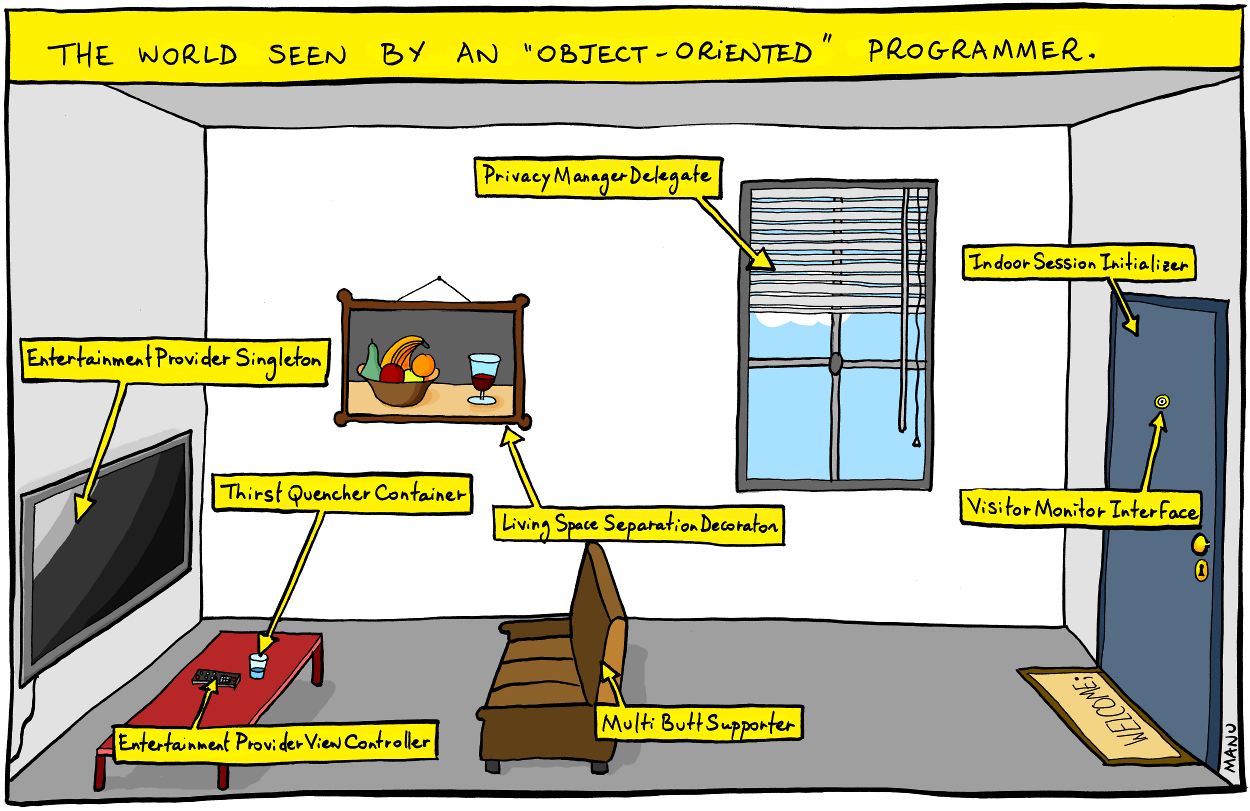
\includegraphics[scale=2]{img/oop.png}
    \end{figure}
\end{frame}

\backupend

\end{document}
